\documentclass[12pt, a4paper]{article}

\usepackage[utf8]{inputenc}
% Limit the page margin to only 1 inch.
\usepackage[margin=1in]{geometry}

%Imports biblatex package
\usepackage[
backend=biber,
style=alphabetic
]{biblatex}
\addbibresource{../../algs4e.bib}

% Enables the `align' environment.
\usepackage{amsmath}
% Provides useful environments, such as:
% - \begin{proof} ...\end{proof}
\usepackage{amsthm}
\usepackage[most]{tcolorbox}

\newtheorem*{proposition}{Proposition}

% Enables using \mathbb{}, for example \mathbb{N} for the set of natural numbers.
\usepackage{amssymb}

% Allows using letters in enumerate list environment. Use, for example:
%\begin{enumerate}[label=(\alph*)]
% ...
%\end{enumerate}
\usepackage[inline]{enumitem}

% Enable importing external graphic files and provides useful commannds, like \graphicspath{}
\usepackage{graphicx}
% Images are located in a directory called images in the current directory.
\graphicspath{{./images/}}

% Make links look better by default.
% See: https://tex.stackexchange.com/questions/823/remove-ugly-borders-around-clickable-cross-references-and-hyperlinks
\usepackage[hidelinks]{hyperref}
\usepackage{xcolor}
\hypersetup{
	colorlinks,
	linkcolor={red!50!black},
	citecolor={blue!50!black},
	urlcolor={blue!80!black}
}


% Code Listings. Source:
% https://stackoverflow.com/questions/3175105/inserting-code-in-this-latex-document-with-indentation
\usepackage{listings}
\usepackage{color}

\definecolor{dkgreen}{rgb}{0,0.6,0}
\definecolor{gray}{rgb}{0.5,0.5,0.5}
\definecolor{mauve}{rgb}{0.58,0,0.82}

\lstset{frame=tb,
	language=Java,
	aboveskip=3mm,
	belowskip=3mm,
	showstringspaces=false,
	columns=flexible,
	basicstyle={\small\ttfamily},
	numbers=none,
	numberstyle=\tiny\color{gray},
	keywordstyle=\color{blue},
	commentstyle=\color{dkgreen},
	stringstyle=\color{mauve},
	breaklines=true,
	breakatwhitespace=true,
	tabsize=3
}

\newcommand{\prob}{\text{P}}
%\newcommand{\complement}{\mathsf{c}}

% Define an environment called "ex" (for Exercise) so that I can do: \begin{ex}{1.5}...\end{ex}
\newenvironment{ex}[2][Exercise]
{\par\medskip\noindent \textbf{#1 #2.}}
{\medskip}

% Define a solution environment, similar to ex (exercise) environment.
\newenvironment{sol}[1][Solution]
{\par\medskip\noindent \textbf{#1.} }
{\medskip}

\begin{document}
	\noindent Sergio E. Garcia Tapia \hfill
	
	\noindent \emph{Algorithms} by Sedgewick and Wayne (4th edition) \cite{sedgewick_wayne}\hfill
	
	\noindent January 16, 2025\hfill 
	\section*{4.3: Minimum Spanning Trees}
	\begin{ex}{1}
		Prove that you can rescale the weights by adding a positive constant to all of them
		or by multiplying them by a positive constant without affecting the MST.
	\end{ex}
	\begin{sol}
		\begin{proof}
			Suppose $G$ is a connected graph. Then $G$ admits an  MST. Let $T$ be
			any MST of $G$.
			
			Let $G_c$ be the graph obtained by adding the positive constant $c$
			to the weight of every edge of $G$. Since the endpoints of the
			edges remain unchanged, it follows that $G_c$ is still connected,
			and thus it admits a spanning tree. In particular, if $T_c$
			is the tree whose edges are the same as $T$ but with weights
			increased by $c$, then $T_c$ is still a spanning tree. To see that it
			is an MST for $G_c$, let $T_c'$ be any other tree spanning tree
			of $G_c$. Let $e_{1,c},\ldots,e_{V-1,c}$ be the edges of $T_c$
			and $f_{1,c},\ldots,f_{V-1,c}$ be the edges of $T_c'$. By definition
			of $G_c$, there are edges $e_k$ and $f_k$ of $G$ satisfying
			\begin{align*}
				w(e_{k,c}')&=w(e_{k}) + c,\\
				w(f_{k,c}')&=w(f_{k}) + c,\\
			\end{align*}
			where $1\leq k\leq V-1$. In particular, the our definition of $T_c$ says that
			$e_1,\ldots,e_{V-1}$ are the edges of $T$, an MST of $G$. Similarly,
			since $T_c'$ is a spanning tree of $G_c$, the edges $f_1,\ldots,f_{V-1}$
			are the same edges but with lower weight. The upshot is that they form
			a spanning tree $T'$ of $G$. By definition of an MST, we know that
			\begin{align*}
				w(T)&\leq w(T')\\
				\sum_{k=1}^{V-1}w(e_k)& \leq \sum_{k=1}^{V-1}w(f_k)\\
				(V-1)\cdot c + \sum_{k=1}^{V-1}w(e_k)& \leq (V-1)\cdot c\sum_{k=1}^{V-1}w(f_k)\\
				\sum_{k=1}^{V-1}(w(e_k) + c)& \leq \sum_{k=1}^{V-1}(w(f_k) + c)\\
				\sum_{k=1}^{V-1}w(e_k')& \leq \sum_{k=1}^{V-1}w(f_k')\\
				w(T_c)&\leq w(T_c')
			\end{align*}
			We conclude that if $T$ is a minimum spanning tree of $G$, the $T_c$ is
			a minimum spanning tree of $G_c$, so the MST is unaffected when all
			edge weights are increased by a positive constant. A similar argument
			works when multiplying by a positive constant.
		\end{proof}
	\end{sol}
	\begin{ex}{2}
		Draw all of the MSTs of the graph depicted in Figure~\ref{fig:ex-02} (all edge weights
		are equal).
		\begin{figure}
			\centering
			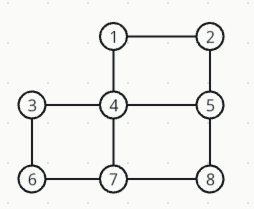
\includegraphics[width=0.2\textwidth]{exercise-02}
			\caption{Undirected edge-weighted graph with all equal weights for Exercise 1.}
			\label{fig:ex-02}
		\end{figure}
	\end{ex}
	\begin{sol}
		Since the graph has $V=8$ vertices, a spanning tree would have $V-1=7$
		edges. The graph is connected with $E=10$ edges, so we need to pick
		$3$ edges to remove. Thus, an upper bound for the number of minimum spanning
		trees is $\binom{10}{3}$. This upper-bound is conservative because we cannot
		just remove \emph{any} edges, given that we also must ensure the graph remains
		connected (else it would not be a spanning tree). Figure~\ref{fig:ex-02-solution} shows
		some, but not all of them.
		\begin{figure}
			\centering
			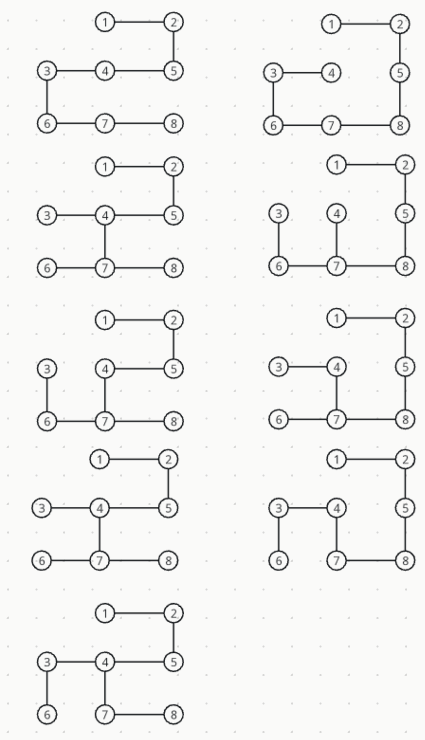
\includegraphics[width=0.4\textwidth]{exercise-02-solution}
			\caption{Some MSTs for the weighted graph in Figure~\ref{fig:ex-02}.}
			\label{fig:ex-02-solution}
		\end{figure}
	\end{sol}
	\begin{ex}{3}
		Show that if a graph's edges all have distinct weights, the MST is unique.
	\end{ex}
	\begin{sol}
		\begin{proof}
			Suppose $T_1$ and $T_2$ are MSTs of a graph $G$ whose edge weights
			are all distinct. Let $e$ be any edge in $T_1$, and suppose that
			$e$ is not in $T_2$. If we add $e$ to $T_2$, then a cycle containing
			$e$ is formed. Let $f$ be any other edge in that cycle, and add
			that edge to $T_1$, thus forming a cycle in $T_1$. By assumption,
			we know that $e$ and $f$ have distinct weights, so without loss
			of generality, suppose $w(e)<w(f)$.
			
			If we remove $f$ from $T_2$, then we eliminate the cycle that was formed
			by adding $e$ to $T_2$, and the tree remains connected. However, now the weight
			of the resulting tree is $w(T_2)-w(e)+w(f)$, which is strictly smaller
			than the weight of $w(T_2)$ because $-w(e)+w(f)<0$. But $T_1$ and
			$T_2$ are MSTs, so this contradicts their minimality.
			
			We conclude that no such each $e$ exists. That is, we do in fact have
			$e\in T_2$. Since $e$ is an arbitrary edge, this hold for every edge of $T_1$.
			A symmetric arguments holds that shows that every edge of $T_2$
			belongs to $T_1$, and hence, $T_1$ and $T_2$ are in fact the
			same tree.
		\end{proof}
	\end{sol}
	\begin{ex}{4}
		Consider the assertion that an edge-weighted graph has a unique MST \emph{only} if
		its edge weights are distinct. Give a proof or a counterexample.
	\end{ex}
	\begin{sol}
		The assertion is false. See Figure~\ref{fig:ex-04}. There are three spanning
		trees:
		\begin{itemize}
			\item The tree with edges \texttt{1-2} and \texttt{1-3}, with a total weight of $15$.
			\item The tree with edges \texttt{1-3} and \texttt{2-3}, with a total weight of $15$.
			\item The tree with edges\texttt{1-2} and \texttt{2-3}, with a total weight of $10$.
		\end{itemize}Though edges \texttt{1-2}
		Among these, only the last one with weight $10$ is an MST, and it is the only MST.
		Note however that not all weights are distinct.
		\begin{figure}
			\centering
			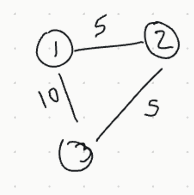
\includegraphics[width=0.2\textwidth]{exercise-04}
			\caption{An undirected weighted tree whose edge weights are not all distinct.}
			\label{fig:ex-04}
		\end{figure}
		
	\end{sol}
	\begin{ex}{5}
		Show that the greedy algorithm is valid even when the edge weights are not distinct.
	\end{ex}
	\begin{sol}
		The statement of the Greedy MST algorithm is:
		\begin{proposition}
			The following method colors black all edges in the MST of any connected
			edge-weighted graph with $V$ vertices: starting with all edges colored gray,
			find a cut with no black crossing edges, color its minimum-weight crossing edge black,
			and continue until $V-1$ edges have been colored black.
		\end{proposition}
		\begin{proof}
			Suppose $G$ is a connected, undirected weighted graph. Start with any cut of
			the graph, and let $e_1$ be \emph{a} crossing edge of minimal weight. Note
			that we are not saying it is \emph{the} crossing edge of minimal weight;
			there may be others with the same weight, but among them we pick $e_1$.
			By the cut property (\textbf{Proposition J}), it belongs to an MST of the graph.
			Suppose that $T$ is an MST of the graph not containing $e_1$.
			By adding $e_1$ to $T$, we create a cycle that contains at least one other edge
			$f$ which crossing the same cut as $e_1$. By the
			minimality of $e_1$, we must have $w(e_1)\leq w(f)$, and since $T$
			is the MST, the possibility $w(e_1)<w(f)$ is impossible (it would imply
			a spanning tree of smaller which, contradicting the minimality of $T$).
			We conclude $w(e_1)=w(f)$. Thus, replacing $f$ by $e_1$, we still have an MST,
			one which $e_1$ belongs to. We color $e_1$ black.
			
			Now suppose that we have colored $k$ edges black, where $1\leq k<V-1$,
			and by the cut property they all belong to \emph{an} (not necessarily
			\emph{the}) MST of the graph. Since $k<V-1$, the tree consisting of the
			$k$ black-colored edges is not spanning, meaning at least one vertex $v$
			is not an endpoint of any of the black-colored edges. In particular, there
			must be a cut with no black crossing edges. For example, one such cut
			consists of precisely the endpoints of the $k$ black-colored edges.
			Since $G$ is connected, there is at least one crossing edge. Let
			$e_{k+1}$ be \emph{any} crossing edge of minimal weight. Let $T_k$ be an
			MST containing all $k$ black-colored edges. If $e_{k+1}$ does not belong
			to $T_k$, then add $e_k$ to $T_k$ to form a cycle. Let $f_{k+1}$ be the other
			edge in the cycle, which must also cross the same cut as $e_{k+1}$. As
			earlier, the minimality of $e_{k+1}$ ensures that $w(e_{k+1})\leq w(f_{k+1})$.
			The minimality of $T_k$ assures us that the possibility $w(f_{k+1})\leq w(e_{k+1})$.
			We conclude that $w(e_{k+1})=w(f_{k+1})$, so we can replace $f_{k+1}$ by
			$e_{k+1}$ and the resulting tree is still a minimal spanning tree. We color
			$e_k$ black.
			
			Now if $V-2$ edges have been colored black, then applying this argument
			again results in a spanning tree consisting of only the $V-1$ black-colored
			edges, which is the MST.
		\end{proof}
	\end{sol}
	\begin{ex}{6}
		Give the MST of the weighted graph obtained by deleting vertex \texttt{7} from
		\texttt{tinyEWG.txt} (see page 604, and Figure~\ref{fig:ex-06}).
		\begin{figure}
			\centering
			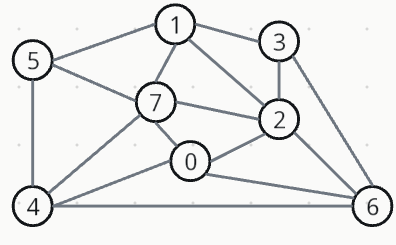
\includegraphics[width=0.3\textwidth]{exercise-06}
			\caption{Undirected weighted graph for \texttt{tinyEWG.txt} (see Exercise 6,
				or page 604).}
			\label{fig:ex-06}
		\end{figure}
		\begin{lstlisting}[language={}]
8
16
4  5  0.35
4  7  0.37
5  7  0.28
0  7  0.16
1  5  0.32
0  4  0.38
2  3  0.17
1  7  0.19
0  2  0.26
1  2  0.36
1  3  0.29
2  7  0.34
6  2  0.40
3  6  0.52
6  0  0.58
6  4  0.93
		\end{lstlisting}
	\end{ex}
	\begin{sol}
		If we delete vertex \texttt{7} and its associated edge, then the remaining
		edges are:
		\begin{lstlisting}[language={}]
4  5  0.35
1  5  0.32
0  4  0.38
2  3  0.17
0  2  0.26
1  2  0.36
1  3  0.29
6  2  0.40
3  6  0.52
6  0  0.58
6  4  0.93
		\end{lstlisting}
		Figure~\ref{fig:ex-06-sol} shows my application of the greedy MST algorithm
		to find the resulting MST when removing vertex \texttt{7}.
		\begin{figure}
			\centering
			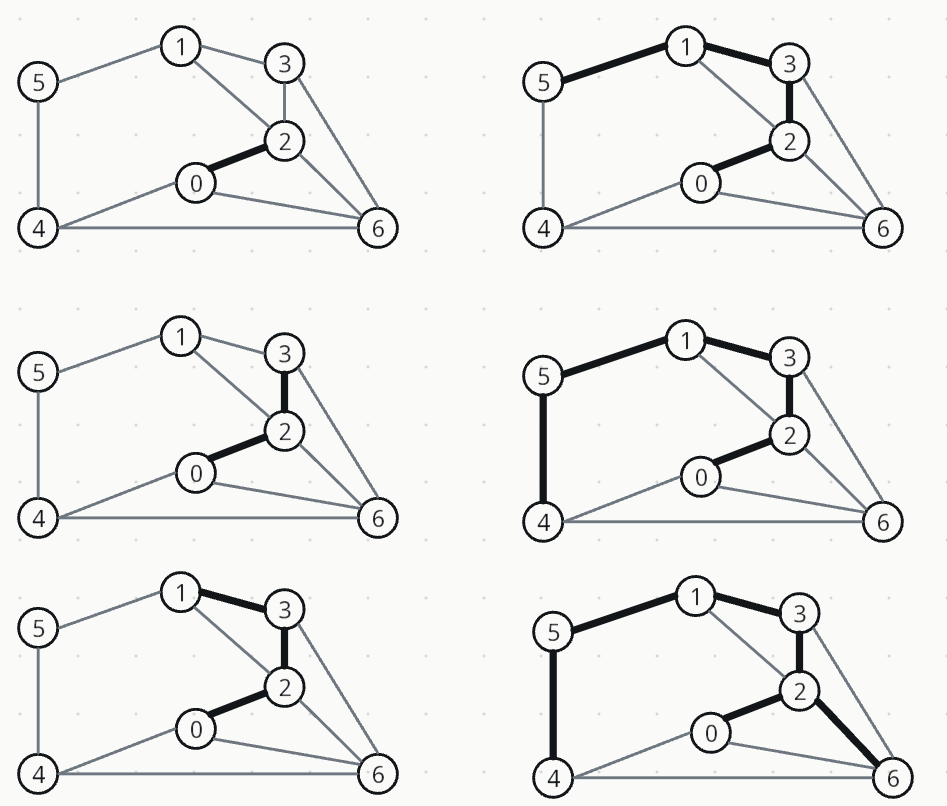
\includegraphics[width=0.6\textwidth]{exercise-06-solution}
			\caption{Applying the Greedy MST algorithm to the tree in Figure~\ref{fig:ex-06}
			after removing vertex \texttt{7}.}
			\label{fig:ex-06-sol}
		\end{figure}
	\end{sol}
	\begin{ex}{7}
		How would you find a \emph{maximum} spanning tree of an edge-weighted graph?
	\end{ex}
	\begin{sol}
		I would apply a version of the greedy MST algorithm that colors black the
		crossing edge of maximal weight (instead of the crossing edge of minimal weight).
	\end{sol}
	\begin{ex}{8}
		Prove the following, known as the \emph{cycle property}: Given any cycle in an
		edge-weighted graph (all edge weights distinct), the edge of maximum weight in
		the cycle does not belong to the MST of the graph.
	\end{ex}
	\begin{sol}
		\begin{proof}
			Let $G$ be a connected undirected edge-weighted graph whose edge weights are
			all distinct. If $G$ has a cycle $\texttt{v}_0\texttt{v}_1\cdots \texttt{v}_k\cdots \texttt{v}_0$,
			let $\texttt{e}_i=\texttt{v}_{i-1}\texttt{v}_{i}$, where $1\leq i\leq k$,
			and $\texttt{e}_{k+1}=\texttt{v}_k\texttt{v}_0$. Without
			loss of generality (perhaps after renaming), say that $\texttt{e}_1$ is the
			edge of maximum weight in the cycle. Given a cut with no black crossing edges
			for which $\texttt{e}_1$ is a crossing edge, I claim that some other edge
			in the cycle must also cross the same cut.
			
			Let $A$ and $B$ be nonempty subsets of the vertices that comprise the cut,
			with $\texttt{v}_0\in A$ and $\texttt{v}_1\in B$. If edges $\texttt{e}_i$
			for $2\leq i\leq {k+1}$ do not cross the cut defined by $A$ and $B$, then
			both endpoints belong to the same side of the cut; that is, they both belong
			to $A$ or they both belong to $B$. Since $\texttt{v}_1\in B$, this implies
			$\texttt{v}_2\in B$, which implies that $\texttt{v}_{i}\in B$ for $2\leq i\leq k$,
			But since $\texttt{e}_{k+1}$ is not a crossing edge either, and since
			$\texttt{v}_k\in B$, this implies that $\texttt{v}_0\in B$ . This is impossible
			because $\texttt{v}_0\in A$, and $A\cap B=\emptyset$ since $A$ and $B$ form
			a partition.
			
			The contradiction implies that there is some edge $\texttt{e}_j$ in the cycle
			distinct from $\texttt{e}_1$ that crosses the same cut as $\texttt{e}_1$.
			By the cut property, the crossing edge of minimum weight belongs to the
			MST. That crossing edge cannot be $\texttt{e}_1$, because $\texttt{e}_j$
			is a crossing edge of smaller weight. Since the cut under consideration
			for which $\texttt{e}_1$ is a crossing edge is arbitrary, we conclude
			that there is no such for which $\texttt{e}_1$ would be the minimum crossing
			edge, and hence, it does not belong to the MST.
		\end{proof}
	\end{sol}
	\begin{ex}{9}
		Implement the constructor for \texttt{EdgeWeightedGraph} that reads an edge-weighted
		graph from the input stream, by suitably modifying the constructor from \texttt{Graph}
		(see page 526).
	\end{ex}
	\begin{sol}
		See \texttt{com.segarciat.algs4.ch4.sec3.ex09}.
	\end{sol}
	\begin{ex}{10}
		Develop an \texttt{EdgeWeightedGraph} implementation for dense graphs that uses an
		adjacency matrix (two-dimensional array of weights) representation. Disallow parallel
		edges.
	\end{ex}
	\begin{sol}
		See \texttt{com.segarciat.algs4.ch4.sec3.ex10}.
	\end{sol}
	\begin{ex}{11}
		Determine the amount of memory used by \texttt{EdgeWeightedGraph} to represent a graph
		with $V$ vertices and $E$ edges, using the memory-cost model of \textbf{Section 1.4}.
	\end{ex}
	\begin{sol}
		First, \texttt{EdgeWeightedGraph} requires 16 bytes of object overhead,
		4 bytes for its \texttt{int E} field, 4 bytes for its \texttt{int V} field,
		and 8 bytes for its reference to \texttt{Bag<Edge>[] adj}. Thus we begin with
		a flat cost of 32 bytes. Next, the array \texttt{adj} itself requires 24
		bytes as flat cost, so now the flat cost is 56 bytes. The array \texttt{adj}
		contains $V$ references to \texttt{Bag<Edge>} objects, each reference is
		$8$ bytes, so that is $8V$ bytes. Now, each \texttt{Bag<Edge>} object
		requires 16 bytes of object overhead, 4 bytes for \texttt{int size},
		8 bytes for the reference to the \texttt{Node first}, and \texttt{4}
		bytes of padding, which is 32 bytes. Since there are $V$ of them, this means
		an additional $32V$ bytes, so now we have $32+40V$ total so far. Now for each
		\texttt{Edge}, we require a \texttt{Node}, which has 16 bytes of overhead,
		8 bytes for the reference to its enclosing class, 8 bytes for the reference
		to \texttt{next}, and 8 bytes for the reference to the item field, for a total
		of 40 bytes. Now, the item referred to by each node is an \texttt{Edge}.
		Moreover, since each edge \texttt{v-w} belongs to both the adjacency list
		of \texttt{v} and the adjacency list of \texttt{w}, the 40 byte cost
		is doubled to 80. However, only one actual edge object exists (both
		nodes refer to the same one). An \texttt{Edge} requires 16 bytes of object
		overhead, 4 bytes for its \texttt{int v} field, 4 bytes for its \texttt{int w}
		field, and 8 bytes for its \texttt{double weight} field, for a total of 32 bytes.
		Hence, each edge requires a total of $40+40+32=112$ bytes.
		
		Now the overall cost is $56+40V+112E$ bytes.
	\end{sol}
	\begin{ex}{12}
		Suppose that a graph has distinct edge weights. Does its lightest edge have to belong
		to the MST? Can its heaviest edge belong to the MST? Does a min-weight edge on
		every cycle have to belong to the MST? Prove your answer to each question or give
		a counterexample.
	\end{ex}
	\begin{sol}
		The lightest edge must belong to the MST. Here's my proof:
		\begin{proof}
			Let \texttt{v-w} be the lightest edge of the tree. Define a cut by
			the singleton set containing \texttt{v} (and its complement). Then
			\texttt{v-w} is a crossing edge for this cut. Since it is the lightest
			edge of the graph, it follows that it is minimum crossing edge for
			this cut, and hence, it must belong to the MST, by the cut property
			(\textbf{Proposition J}).
		\end{proof}
		Yes, the heaviest edge may belong to the MST. Consider the graph on
		Figure~\ref{fig:ex-12-heaviest-edge}. We see that \texttt{3-4} is the heaviest edge,
		but it is also the only edge to vertex \texttt{4}. Therefore, any spanning
		tree must contain \texttt{4}, including the MST.
		\begin{figure}
			\centering
			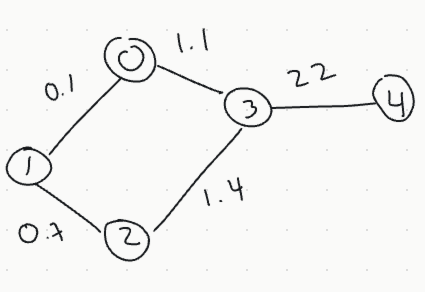
\includegraphics[width=0.3\textwidth]{exercise-12-heaviest-edge}
			\caption{A weighted graph whose heaviest edge must belong to the MST.}
			\label{fig:ex-12-heaviest-edge}
		\end{figure}
		
		Figure~\ref{fig:ex-12-cycle-counterexample} shows an example of a graph $G$
		with a weighted edge \texttt{2-3} that has minimum weight in the cycle
		\texttt{2-3-4}. However, \texttt{2-3} does not belong to the MST. To see this,
		note that since all the weights of $G$ are distinct, the MST is unique.
		If we apply Prim's algorithm starting at vertex \texttt{0}, we would add
		\texttt{0-1}, followed by \texttt{1-2}, followed by \texttt{1-2},
		followed by \texttt{3-4}, completing the MST.
		\begin{figure}
			\centering
			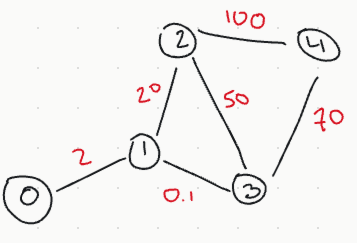
\includegraphics[width=0.3\textwidth]{exercise-12-cycle-lightest-edge-counter}
			\caption{A weighted graph with a min-weight edge in a cycle.}
			\label{fig:ex-12-cycle-counterexample}
		\end{figure}
	\end{sol}
	\begin{ex}{13}
		Give a counterexample that shows why the following strategy does not necessarily
		find the MST: ``Start with any vertex as a single-vertex MST, the add \texttt{V-1}
		edges to it, always taking next a min-weight edge incident to the vertex most
		recently added to the MST."
	\end{ex}
	\begin{sol}
		The problem is we cannot guarantee that the min-weight edge incident on
		the most recently added vertex is necessarily the best way to connect
		the vertex on the other endpoint of the edge to the tree,
		If we apply the algorithm to the graph depicted in Figure~\ref{fig:ex-13},
		starting at vertex \texttt{1}, we would pick edge \texttt{1-3} first,
		and since \texttt{3} is the most recently added vertex, we need to pick
		the minimum weight edge incident to \texttt{3}. The only edge incident to
		\texttt{3} that is not in the tree is \texttt{3-4}, and then finally we would
		add edge \texttt{4-2}. However, this is not the MST. In particular, the spanning
		tree consisting of edges \texttt{1-3}, \texttt{1-2}, and \texttt{2-4}
		is the MST.
		\begin{figure}
			\centering
			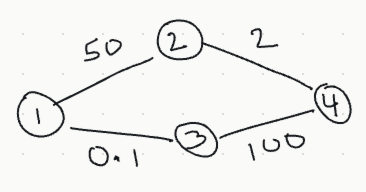
\includegraphics[width=0.3\textwidth]{exercise-13}
			\caption{Counterexample for Exercise 13.}
			\label{fig:ex-13}
		\end{figure}
	\end{sol}
	\begin{ex}{14}
		Given an MST for an edge-weighted graph $G$, suppose that an edge in $G$ that
		does not disconnect $G$ is deleted. Describe how to find an MST for the new graph
		in time proportional to $E$.
	\end{ex}
	\begin{sol}
		Let $T$ be the MST of $G$ in question, and let $e$ be the edge removed from $G$.
		First, we check whether $e$ belongs to $T$. If not, then $T$ is still a spanning
		tree of the new graph. Moreover, if $T'$ were a spanning tree of smaller
		weight for the new graph, then it would be a spanning tree of $G$ also,
		which would contradict the minimality of $T$.
		
		Now suppose $e$ does belong to $T$. Then $e$ disconnects $T$. We can use depth-first
		search to find the two connected components of $T$, 
	\end{sol}
	
	\pagebreak
	\printbibliography
\end{document}